\documentclass[letterpaper]{article}
\usepackage[square,sort,comma,numbers]{natbib}
\usepackage{array}
%====================================================================%
../../../../tex/scufftex.tex
\graphicspath{{figures/}}
\renewcommand{\wt}{\widetilde}
\newcommand{\vbCSlash}{\backslash\hspace{-0.085in}\vb C}
\newcommand{\JSlash}{\backslash\hspace{-0.085in}J}

%------------------------------------------------------------
%------------------------------------------------------------
%- Special commands for this document -----------------------
%------------------------------------------------------------
%------------------------------------------------------------

%------------------------------------------------------------
%------------------------------------------------------------
%- Document header  -----------------------------------------
%------------------------------------------------------------
%------------------------------------------------------------
\title {Implicit handling of multilayered material substrates
        in full-wave {\sc scuff-em} calculations
       }
\author {Homer Reid}
\date {August 16, 2017}

%------------------------------------------------------------
%------------------------------------------------------------
%- Start of actual document
%------------------------------------------------------------
%------------------------------------------------------------

\begin{document}
\pagestyle{myheadings}
\markright{Homer Reid: Implicit substrates in full-wave {\sc scuff-em}}

\maketitle

\tableofcontents

%====================================================================%
%====================================================================%
%====================================================================%
\newpage
\section{Overview}

In a 
previous memo\footnote{``Implicit handling of multilayered dielectric
substrates in {\sc scuff-static}''} I
considered {\sc scuff-static} electrostatics calculations
in the presence of a multilayered dielectric substrate.
In this memo I extend that discussion to the case of
\textit{full-wave} (i.e. nonzero frequencies beyond the
quasistatic regime) scattering calculations in the
{\sc scuff-em} core library.

%%%%%%%%%%%%%%%%%%%%%%%%%%%%%%%%%%%%%%%%%%%%%%%%%%%%%%%%%%%%%%%%%%%%%%
%%%%%%%%%%%%%%%%%%%%%%%%%%%%%%%%%%%%%%%%%%%%%%%%%%%%%%%%%%%%%%%%%%%%%%
%%%%%%%%%%%%%%%%%%%%%%%%%%%%%%%%%%%%%%%%%%%%%%%%%%%%%%%%%%%%%%%%%%%%%%
\subsubsection*{Substrate geometry}

As shown in Figure \ref{SubstrateGeometryFigure}, I consider
a multilayered substrate consisting of $N$ material layers
possibly terminated by a perfectly-conducting ground plane.
The uppermost layer (layer 1) is the infinite half-space
above the substrate.
The $n$th layer
has relative permittivity and permeability $\epsilon_n,\mu_n$,
and its lower surface lies at $z=z_n$.
The ground plane, if present,
lies at $z\equiv z\subt{N}\equiv z\subt{GP}$.
If the ground plane is absent, layer $N$ is an
infinite half-space\footnote{As in the electrostatic case,
this means that a finite-thickness substrate consisting of
$N$ material layers is described as a stack of $N+1$ layers
in which the bottommost layer is an infinite vacuum half-space.}
($z\subt{N}=-\infty$).
%####################################################################%
%####################################################################%
%####################################################################%
\begin{figure}[!]
\begin{center}
\resizebox{\textwidth}{!}{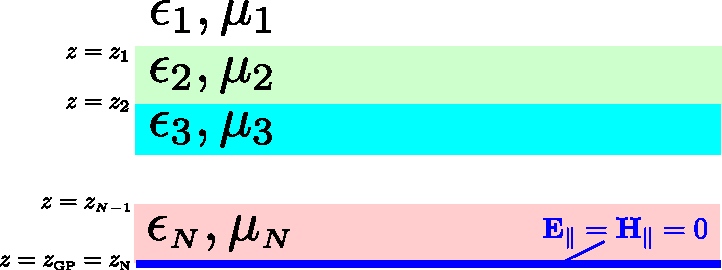
\includegraphics{MultilayerSubstrate.pdf}}
\caption{Geometry of the layered substrate.
The $n$th layer 
has relative permittivity and permeability $\epsilon_n,\mu_n$,
and its lower surface lies at $z=z_n$. The ground plane, if present,
lies at $z=z\subt{GP}.$
}
\label{SubstrateGeometryFigure}
\end{center}
\end{figure}
%####################################################################%

%%%%%%%%%%%%%%%%%%%%%%%%%%%%%%%%%%%%%%%%%%%%%%%%%%%%%%%%%%%%%%%%%%%%%%
%%%%%%%%%%%%%%%%%%%%%%%%%%%%%%%%%%%%%%%%%%%%%%%%%%%%%%%%%%%%%%%%%%%%%%
%%%%%%%%%%%%%%%%%%%%%%%%%%%%%%%%%%%%%%%%%%%%%%%%%%%%%%%%%%%%%%%%%%%%%%
\subsubsection*{Mechanics of implementation in {\sc scuff-em}}

The full-wave substrate implementation in {\sc scuff-em} involves multiple 
working parts. 

%####################################################################%
%####################################################################%
%####################################################################%
\newpage
\section{Computation of Fourier-space DGF}
\label{GTwiddleSection}

%####################################################################%
%####################################################################%
%####################################################################% \newpage
\section{Reduction of 2D integrals over $\vb q$ to 1D integrals over $q$}
\label{TwoD2OneDSection}

%####################################################################%
%####################################################################%
%####################################################################%
\newpage
\section{Evaluation of 1D integrals}

%####################################################################%
%####################################################################%
%####################################################################%
\newpage
\section{Substrate contributions to panel and panel-panel integrals}

\begin{align*}
 \bmc G\supt{PQ}(\rho, \theta, z\subt{D}, z\subt{S})
  &= \sum_{\nu p} 
      g^{\text{\tiny PQ}\nu p}(\rho, z\subt{D}, z\subt{S})
      \vbLambda^{\text{\tiny PQ}\nu p}(\theta)
\label{GPQExpression}
\\
g^{\text{\tiny PQ}\nu p}(\rho)
&=\int \frac{qdq}{(2\pi)}
       \wt{g}^{\text{\tiny PQ}\nu p}(q)
        J_\nu(q\rho) e^{i\alpha(q,z\subt{D},z\subt{S})} 
        \vbLambda^{\text{\tiny PQ}\nu p}(\theta)
\end{align*}

\begin{align*}
M\supt{PQ}_{\alpha\beta}
 \VMV{\vb b_\alpha}{\bmc G\supt{PQ}}{\vb b_\beta}
\end{align*}

%####################################################################%
%####################################################################%
%####################################################################%
\end{document}
